\section{
  \texorpdfstring{数值方法介绍} % 正文和目录中显示的标题
  {\thesection 数值方法介绍} % 书签页中显示的标题
}
\label{sec:数值方法介绍}

目前船舶与海洋工程领域的势粘流耦合方法研究主要集中于非线性波浪数值模拟、极端波浪演化与传播和船舶耐波性与操纵性等问题，%
而对于砰击、上浪等涉及强非线性自由液面现象的问题研究较少。%
因此本文针对海上浮式平台遭受波浪砰击、上浪等强非线性自由液面运动问题，%
基于非线性势流高阶谱方法、边界元方法以及无网格光滑粒子流体动力学方法开展势粘流耦合方法的研究。%

本章首先分别介绍几种势粘流数值方法的基本理论和所采用的求解器，包括：%
高阶谱方法的基本理论以及所采用的开源求解器HOS-NWT数值水池，%
二维时域Rankine源边界元方法以及基于该方法所实现的数值水池，%
光滑粒子流体动力学方法和改进的$\delta^+$-SPH模型。%
最后通过规则波和不规则波的数值波浪模拟分析了几种方法的收敛性和准确性，并对不同方法结果进行了对比。

\subsection{
  \texorpdfstring{高阶谱方法} % 正文和目录中显示的标题
  {\thesubsection 高阶谱方法} % 书签页中显示的标题
}
\label{ssec:高阶谱方法}

\subsubsection{
  \texorpdfstring{高阶谱方法基础理论} % 正文和目录中显示的标题
  {\thesubsubsection 高阶谱方法基础理论} % 书签页中显示的标题
}
\label{sssec:高阶谱方法基础理论}

高阶谱方法(High Order Spectral，简称HOS)是一种基于势流理论的伪谱方法，%
最早由Dommermuth和Yue\cite{dommermuthHighorderSpectralMethod1987a}以及%
West等人\cite{westNewNumericalMethod1987a}分别提出。%
在HOS方法中，流体满足无粘不可压以及无旋流假设，并且波陡符合小量假设。%
流动通过速度势$\phi\left(\bm{x},z,t\right)$进行描述，其满足Laplace方程、自由液面运动学和动力学条件：
\begin{equation}
  \nabla^2\phi\left(\bm{x},z,t\right) = 0
  \label{eq:HOS-Laplace}
\end{equation}
\begin{equation}
  \frac{\partial \eta}{\partial t} + \frac{\partial \phi}{\partial \bm{x}}\frac{\partial \eta}{\partial \bm{x}} %
  - \frac{\partial \phi}{\partial z} = 0,\quad z = \eta
  \label{eq:HOS-KFBC}
\end{equation}
\begin{equation}
  \frac{\partial \phi}{\partial t} %
  + \frac{1}2 \left[\left(\frac{\partial \phi}{\partial \bm{x}}\right)^2 %
  + \frac{\partial \phi}{\partial z}^2\right] + g\eta = 0,\quad z = \eta
  \label{eq:HOS-DFBC}
\end{equation}
式中：$\eta = \left(\bm{x},t\right)$为波高，$g$为重力加速度。%
$\bm{x} = \left(x,y\right)$为水平方向位置向量(二维情况下不考虑$y$方向)，$z$为竖直方向坐标，$t$为时间。

根据Zakharov方程\cite{zakharovStabilityPeriodicWaves1968}，将自由面上的速度势定义为：
\begin{equation}
  \phi^s\left(\bm{x},t\right) = \phi\left[\bm{x},\eta\left(\bm{x},t\right),t\right]
  \label{eq:HOS-Zakharov}
\end{equation}

将\cref{eq:HOS-Zakharov}带入\cref{eq:HOS-KFBC}和\cref{eq:HOS-DFBC}中可得关于$\phi^s$和$\eta$的边界控制方程：
\begin{equation}
  \frac{\partial \eta}{\partial t} + \frac{\partial\phi^s}{\partial \bm{x}}\frac{\partial\eta}{\partial \bm{x}} %
  - \left(1 + \frac{\partial\eta}{\partial \bm{x}}\frac{\partial\eta}{\partial \bm{x}}\right)%
  \frac{\partial\phi^s}{\partial z} = 0,\quad z = \eta
  \label{eq:HOS-BCE-phi}
\end{equation}
\begin{equation}
  \frac{\partial\phi^s}{\partial t} + g\eta %
  + \frac{1}2\frac{\partial\phi^s}{\partial\bm{x}}\frac{\partial\phi^s}{\partial\bm{x}} %
  - \frac{1}2\left(1 + \frac{\partial\eta}{\partial \bm{x}}\frac{\partial\eta}{\partial \bm{x}}\right) %
  \left(\frac{\partial\phi^s}{\partial z}\right)^2 = 0,\quad z = \eta
  \label{eq:HOS-BCE-eta}
\end{equation}

假设$\phi$和$\eta$为$O\left(\epsilon\right)$阶小量，并将速度势以波陡为小量进行$M$阶摄动展开得到：
\begin{equation}
  \phi\left(\bm{x},z,t\right) = \sum_{m=1}^{M}\phi^{\left(m\right)}\left(\bm{x},z,t\right)
  \label{eq:HOS-perturbation}
\end{equation}

而后将摄动展开的每一项$\phi^{\left(m\right)}$进行泰勒展开，并代入\cref{eq:HOS-perturbation}得到：
\begin{equation}
  \phi^s\left(\bm{x},t\right) = \phi\left(\bm{x},\eta,t\right) %
  = \sum_{m=1}^{M}\sum_{k=0}^{M-m}\frac{\eta^k}{k!}\frac{\partial^k}{\partial z^k} %
  \phi^{\left(m\right)}\left(\bm{x},0,t\right)
  \label{eq:HOS-Taylor}
\end{equation}

将\cref{eq:HOS-Taylor}展开并合并同阶项，整理可得到$\phi^{\left(m\right)}$在平均水面处的边界条件方程：
\begin{eqnarray}
  \phi^{\left(m\right)}\left(\bm{x},0,t\right) = R^{\left(m\right)}, \quad m = 1, 2, 3, \cdots, M
\end{eqnarray}
其中：
\begin{subequations}
  \begin{gather}
    R^{\left(1\right)} = \phi^s \\
    R^{\left(m\right)} = - \sum_{k=1}^{m-1}\frac{\eta^k}{k!}\frac{\partial^k}{\partial z^k}\phi^{m-k}\left(\bm{x},0,t\right), %
    \quad m = 1, 2, 3, \cdots, M
  \end{gather}
\end{subequations}
通过给定的初始自由液面边界条件$\phi^s$和$\eta$，可以依上式递推得出摄动展开的各阶项$\phi^{\left(m\right)}$。

在HOS方法中，空间导数的求解在傅里叶频域空间进行，而一般变量的求解在物理空间进行。%
为了实现这点，将摄动展开的各阶项$\phi^{\left(m\right)}$进行模态展开得到：
\begin{equation}
  \phi^{\left(m\right)}\left(\bm{x},z,t\right) = \sum_{n=0}^{m}\phi_n^{\left(m\right)}\left(t\right) %
  \psi_n\left(\bm{x},z\right)
  \label{eq:HOS-modes}
\end{equation}
其中$\psi_n\left(\bm{x},z\right)$为满足Laplace方程和各边界条件的基函数。%
对于无限水深和有限水深问题分别取不同的基函数：

无限水深：
\begin{equation}
  \phi^{\left(m\right)}\left(\bm{x},z,t\right) = \sum_{n=0}^{m} \phi_n^{\left(m\right)}\left(t\right) %
  \exp\left[\left|\bm{k}_n\right|z + i\bm{k}_n\cdot \bm{x}\right]
\end{equation}

有限水深：
\begin{equation}
  \phi^{\left(m\right)}\left(\bm{x},z,t\right) = \sum_{n=0}^{m} \phi_n^{\left(m\right)}\left(t\right) %
  \frac{\cosh\left[\left|\bm{k}_n\right|\left(z + h\right)\right]}{\cosh\left(\left|\bm{k}_n\right|h\right)}%
  \exp\left(i\bm{k}_n\cdot \bm{x}\right)
\end{equation}
式中：$\bm{k}_n = \left(k_x,k_y\right)$为波数向量，$\left|\bm{k}_n\right| = \sqrt{{k_x}^2 + {k_y}^2}$，%
$k_x = 2\pi i/L_x$，$k_y = 2\pi i/L_y$，其中$i$、$j$、$L_x$、$L_y$分别表示$x$、 $y$方向上的模态数和长度%
(二维情况下不考虑$y$方向)，在数值计算中会对模态数进行截断。

将\cref{eq:HOS-modes}带入\cref{eq:HOS-Taylor}并给出自由面速度势在$z$方向上的导数：
\begin{equation}
  \phi_z\left(\bm{x},\eta,t\right) = \sum_{m=1}^{M}\sum_{k=0}^{M-m}\frac{\eta^k}{k!}%
  \sum_{n=1}^{N} \phi_n^{\left(m\right)}\left(t\right) \frac{\partial^{k+1}}{\partial z^{k+1}}%
  \psi_n\left(\bm{x},0\right)
  \label{eq:HOS-derivative-z}
\end{equation}
其中$\phi_n^{\left(m\right)}\left(t\right)$可以通过%
对$\phi^{\left(m\right)}$进行快速傅里叶变换(Fast Fourier Transform，简称FFT)得到，%
从而实现在傅里叶频域空间对速度势空间导数进行求解。

将\cref{eq:HOS-derivative-z}带入自由液面边界条件\cref{eq:HOS-BCE-phi}和%
\cref{eq:HOS-BCE-eta}可得关于$\phi^s$和$\eta$的方程：
\begin{subequations}
  \begin{gather}
    \frac{\partial n}{\partial t} %
    + \left(\frac{\partial\phi^s}{\partial\bm{x}} \frac{\partial\eta}{\partial\bm{x}}\right) %
    \left[\sum_{m=1}^{M}\sum_{k=0}^{M-m}\frac{\eta^k}{k!}%
    \sum_{n=1}^{N} \phi_n^{\left(m\right)}\left(t\right) \frac{\partial^{k+1}}{\partial z^{k+1}}%
    \psi_n\left(\bm{x},0\right)\right] = 0 %
    \label{eq:HOS-ODE-phi} \\
    %
    \frac{\partial\phi^s}{\partial t} + g\eta %
    + \frac{1}2\frac{\partial\phi^s}{\partial\bm{x}}\frac{\partial\phi^s}{\partial\bm{x}} %
    - \frac{1}2\left(1 + \frac{\partial\eta}{\partial \bm{x}}\frac{\partial\eta}{\partial \bm{x}}\right) %
    \left[\sum_{m=1}^{M}\sum_{k=0}^{M-m}\frac{\eta^k}{k!}%
    \sum_{n=1}^{N} \phi_n^{\left(m\right)}\left(t\right) \frac{\partial^{k+1}}{\partial z^{k+1}}%
    \psi_n\left(\bm{x},0\right)\right]^2 = 0 %
    \label{eq:HOS-ODE-eta}
  \end{gather}
\end{subequations}

当给定初始自由液面边界条件$\phi^s$和$\eta$时，%
通过对\cref{eq:HOS-ODE-phi}和\cref{eq:HOS-ODE-eta}进行积分可以实现时间上的步进。%
由于HOS方法在数值计算过程中引入了FFT方法，因此该数值方法是伪谱法，%
并且具有较高的计算效率和精度\cite{seiffertSimulationBreakingWaves2018}

\subsubsection{
  \texorpdfstring{HOS-NWT数值水池} % 正文和目录中显示的标题
  {\thesubsubsection HOS-NWT数值水池} % 书签页中显示的标题
}
\label{sssec:HOS-NWT数值水池}

本文所采用的HOS求解器是法国南特中央理工大学的Ducrozet等人发布的%
开源数值水池HOS-NWT\cite{ducrozetModifiedHighOrderSpectral2012}，%
该求解器能够实现最高达到三阶非线性的数值造波，其基本理论可见\cref{sssec:高阶谱方法基础理论}所述。%
在数值水池造波过程中，需要考虑造波机运动所产生的造波边界条件和消波区域的设置，如\cref{fig:ch2-HOS-NWT}所示。%
\begin{myfigure}
  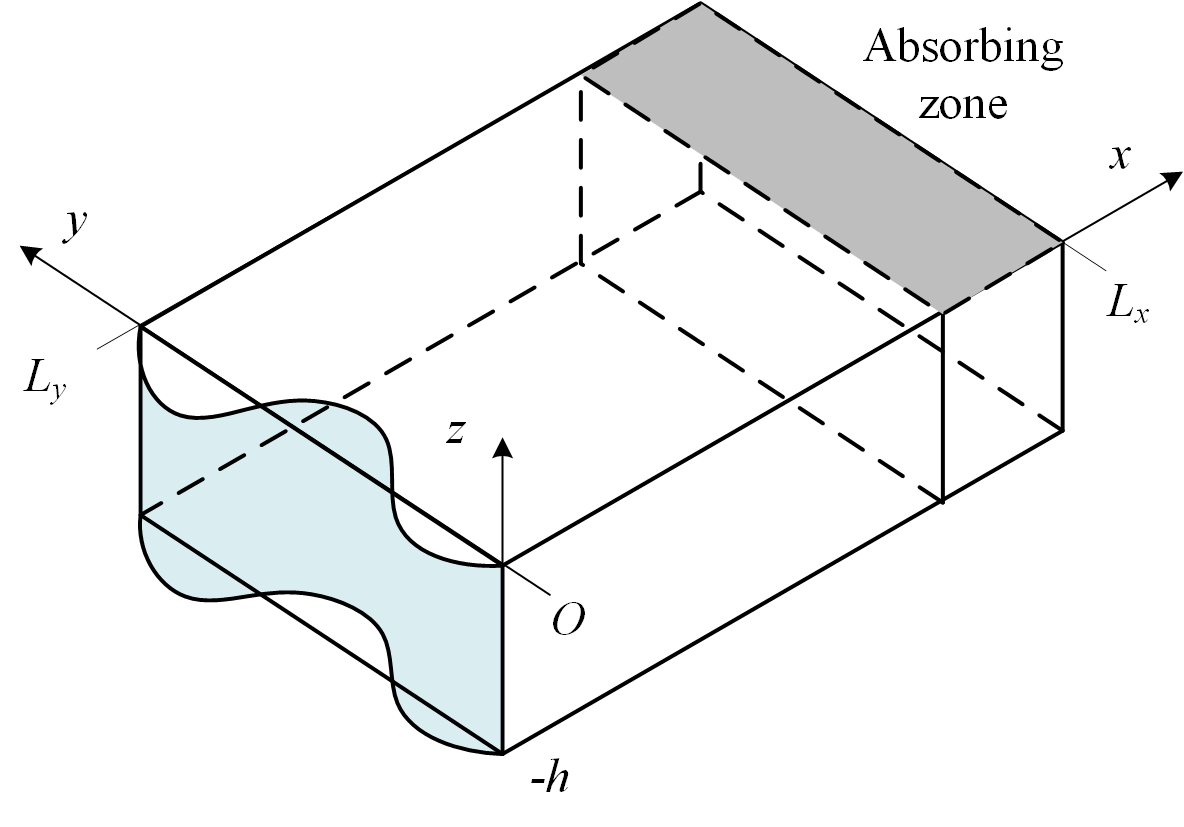
\includegraphics[width=0.5\textwidth]{figures/ch2-HOS-NWT.png}
  \caption{HOS-NWT数值水池方案及其坐标系}
  \label{fig:ch2-HOS-NWT}
\end{myfigure}

其中消波区域$\Omega_{\rm{Absorbing}}$是通过对自由液面上的压力进行局部修正来实现的，%
修正压力为\cite{bonnefoyFullyspectral3DTimedomain2006}：
\begin{equation}
  p^{*} = \rho\nu\left(x\right) \frac{\partial\phi}{\partial\bm{x}} \cdot \bm{n}, \quad z = \eta
\end{equation}
式中：$\nu\left(x\right)$为修正函数，$\bm{n}$为自由液面的法向量。

下面简单介绍在HOS-NWT数值水池中造波边界条件的处理。

将造波机的运动描述为壁面在$x$方向上的运动$X = X\left(y,z,t\right)$(二维情况下不考虑$y$方向)，则造波边界条件可以表达为：
\begin{equation}
  \frac{\partial X}{\partial t} = \frac{\partial\phi}{\partial x} %
  - \nabla_{yz}X \cdot \nabla_{yz}\phi, x = X\left(y,z,t\right)
\end{equation}
式中：$\nabla_{yz} = \left(\dfrac{\partial}{\partial y}, \dfrac{\partial}{\partial z}\right)$。

HOS-NWT通过引入附加速度势处理该造波边界条件，将总速度势分解为两个分量$\phi = \phi_{\rm{spec}} + \phi_{\rm{add}}$。%
其中$\phi_{\rm{spec}}$为描述固定壁面水池(即$X = 0$时)自由液面演化的速度势，%
而$\phi_{\rm{add}}$为考虑造波边界条件的附加速度势。 %
除了需要满足Laplace方程和壁面边界条件外，还需要满足造波边界条件。%
将自由面上的速度势$\phi_{\rm{spec}}$定义为$\phi^s\left(\bm{x},t\right) = \phi_{\rm{spec}}\left(\bm{x},\eta,t\right)$，%
则自由液面边界条件\cref{eq:HOS-BCE-phi}和\cref{eq:HOS-BCE-eta}由于$\phi_{\rm{add}}$的引入被改写为：
\begin{equation}
  \left\{
    \begin{aligned}
    \frac{\partial\eta}{\partial t} =& %
    \left(1 + \frac{\partial\eta}{\partial \bm{x}}\frac{\partial\eta}{\partial \bm{x}}\right) %
    \frac{\partial\phi^s}{\partial z} %
    - \frac{\partial\left(\phi^s + \phi_{\rm{add}}\right)}{\partial\bm{x}} \frac{\partial\eta}{\partial\bm{x}} %
    + \frac{\partial\phi_{\rm{add}}}{\partial z} \\
    %
    \frac{\partial\phi^s}{\partial t} =& - g\eta %
    - \frac{1}2 \frac{\partial\phi^s}{\partial\bm{x}} \frac{\partial\phi^s}{\partial\bm{x}} %
    + \frac{1}2\left(1 + \frac{\partial\eta}{\partial \bm{x}}\frac{\partial\eta}{\partial \bm{x}}\right) %
    \left(\frac{\partial\phi^s}{\partial z}\right)^2 \\
    &- \frac{\partial\phi^s}{\partial\bm{x}} \frac{\partial\phi_{\rm{add}}}{\partial\bm{x}} %
    - \frac{1}2 \frac{\partial\phi_{\rm{add}}}{\partial\bm{x}}\frac{\partial\phi_{\rm{add}}}{\partial\bm{x}} %
    - \frac{\partial\phi_{\rm{add}}}{\partial t} - \nu \frac{\partial\eta}{\partial t}
    \end{aligned}
  \right. %
  , \quad z = \eta
  \label{eq:HOS-NWT-FBC}
\end{equation}

因此$\phi_{\rm{spec}}$和$\phi_{\rm{add}}$分别满足下列的边界条件：
\begin{equation}
  \left\{
    \begin{aligned}
      & \nabla^2\phi_{\rm{spec}} = 0, \quad \left(x,y,z\right) \in \Omega \\
      %
      & \frac{\partial \phi_{\rm{spec}}}{\partial n} = 0, \quad x = 0, L_x; y = 0; z = -h \\
      %
      & \text{引入}\phi_{\rm{add}}\text{的自由液面边界条件}, \text{即\cref{eq:HOS-NWT-FBC}}, %
      \quad z = \eta\left(\bm{x},t\right)
    \end{aligned}
  \right. 
  \label{eq:HOS-NWT-BC-spec}
\end{equation}
\begin{equation}
  \left\{
    \begin{aligned}
      & \nabla^2\phi_{\rm{add}} = 0, \quad \left(x,y,z\right) \in \Omega \\
      %
      & \frac{\partial \phi_{\rm{add}}}{\partial n} = \quad x = 0, L_x; y = 0; z = -h \\
      %
      & \frac{\partial \phi_{\rm{add}}}{\partial X} + \nabla_{yz}X \cdot \nabla_{yz}\phi_{\rm{add}} = %
      \frac{\partial X}{\partial t} \frac{\phi_{\rm{spec}}}{\partial X} %
      - \nabla_{yz}X \cdot \nabla_{yz}\phi_{\rm{spec}}, \quad x = X\left(y,z,t\right)
    \end{aligned}
  \right. 
  \label{eq:HOS-NWT-BC-add}
\end{equation}

根据\cref{eq:HOS-NWT-BC-spec}和\cref{eq:HOS-NWT-BC-add}，数值波浪模拟被分解为两个问题。%
首先求解出满足造波边界条件的附加速度势$\phi_{\rm{add}}$，%
而后根据改写的自由液面边界条件\cref{eq:HOS-NWT-FBC}求解$\phi_{\rm{spec}}$，从而实现整个问题的求解。%

HOS-NWT中采用SWEET模型\cite{bonnefoyFullyspectral3DTimedomain2006,bonnefoyFullyspectral3DTimedomain2006a}%
对附加速度势进行求解，%
并且Guillaume等人\cite{ducrozetModifiedHighOrderSpectral2012} 将该模型的造波边界条件推广到了三阶非线性。%
计算中采用自适应步长的四阶Runge–Kutta Cash–Karp时间推进格式\cite{cashVariableOrderRungeKutta1990}。%

在所发布的HOS-NWT求解器中，计算的初始条件为波浪信息，%
如规则波的周期和波高、不规则波的波浪谱等，其中还内置了JONSWAP波浪谱可以用于计算使用。%
为了便于与试验或其他数值方进行对比，本文在HOS-NWT求解器的基础上，%
添加了以造波机运动作为边界条件的功能，从而能够根据造波机的运动时程实现数值造波。

\subsection{
  \texorpdfstring{边界元方法} % 正文和目录中显示的标题
  {\thesubsection 边界元方法} % 书签页中显示的标题
}
\label{ssec:边界元方法}

边界元方法(Boundary Element Method，简称BEM)是十分成熟的势流方法。%
本文参考文献\parencite{grilliNumericalModelingWave1996,SunErWeiZiYouMianTiaoJianHeFuSheTiaoJianDeShuZhiMoNi2004}%
实现了基于二维时域Rankine源边界元法的数值波浪水池，下面简单介绍边界元方法的基础理论。

\subsubsection{
  \texorpdfstring{边界积分方程} % 正文和目录中显示的标题
  {\thesubsubsection 边界积分方程} % 书签页中显示的标题
}
\label{sssec:边界积分方程}

在无粘、不可压以及无旋流假设下，流动可以通过速度势$\phi$进行描述，%
控制方程为Laplace方程\cref{eq:HOS-Laplace}，通过格林第三公式可以将其转换为边界积分方程：
\begin{equation}
  \alpha\left(P\right) \phi\left(P,t\right) %
  + \int_{\Gamma} \left[\phi\left(Q,t\right) \frac{\partial G_{PQ}}{\partial n_Q} %
  - \frac{\partial \phi\left(Q,t\right)}{\partial n_Q}G_{PQ}\right] {\rm{d}} l = 0
  \label{eq:BEM-BIE}
\end{equation}
其中$G$为二维Rankine源格林函数：
\begin{equation}
  \left\{
    \begin{aligned}
      & G_{PQ} = G\left(P,Q\right) = \ln\frac{1}{\bm{r}_{PQ}} %
      = \ln \frac{1}{\sqrt{\left(x_P - x_Q\right)^2 + \left(z_P - z_Q\right)^2}} \\
      % 
      & \frac{\partial G_{PQ}}{\partial n_Q} = -\frac{\left(\bm{r}_Q - \bm{r}_P\right)}{{r_{PQ}}^2} \cdot n_Q
    \end{aligned}
  \right.
\end{equation}
式中：$P$，$Q$分别表示流场中的场点和边界上的源点，$r$为位置矢量，$n$为流场边界的外法向。%
$\alpha\left(P\right)$为场点处的空间角，当$P$位于流场内部，$\alpha\left(P\right) = 2\pi$；%
当$P$位于流场边界，$\alpha\left(P\right)$为边界在该点的张开角。%
对于直线、一阶或高阶光滑曲线等连续边界，$\alpha\left(P\right) = \pi$。

对于二维有限水深的数值波浪水池，需要考虑造波机边界$\Gamma_w$、固壁边界$\Gamma_s$和自由液面边界$\Gamma_f$这三种边界。%
其中造波机边界$\Gamma_w$和固壁边界$\Gamma_s$的边界条件为Newmann边界条件，而自由液面边界$\Gamma_f$为Dirichlet边界条件。%
因此根据各个边界上所提供的边界条件不同，离散的边界积分方程可以分别写为：
\begin{subequations}
  \begin{align}
    \begin{aligned}
      \alpha_i\phi_i + \sum_{P_j\in \Gamma_w\cap\Gamma_s}\phi_j %
      \int_{\Delta\Gamma} \frac{\partial G_{ij}}{\partial n_j} {\rm{d}} l %
      - \sum_{P_j\in \Gamma_f}\frac{\partial \phi_j}{\partial n_j} %
      \int_{\Delta\Gamma} G_{ij} {\rm{d}} l =& \\%
      \sum_{P_j\in \Gamma_w\cap\Gamma_s}\frac{\partial \phi_j}{\partial n_j} %
      \int_{\Delta\Gamma} G_{ij} {\rm{d}} l %
      - \sum_{P_j\in \Gamma_f}\phi_j & %
      \int_{\Delta\Gamma} \frac{\partial G_{ij}}{\partial n_j} {\rm{d}} l %
    \end{aligned}, \quad & P_i \in \Gamma_w \cap \Gamma_s
    \label{eq:BEM-discrete-BIE-1} \\
    %
    \begin{aligned}
      \sum_{P_j\in \Gamma_w\cap\Gamma_s}\phi_j %
      \int_{\Delta\Gamma} \frac{\partial G_{ij}}{\partial n_j} {\rm{d}} l %
      - \sum_{P_j\in \Gamma_f}\frac{\partial \phi_j}{\partial n_j} %
      \int_{\Delta\Gamma} G_{ij} {\rm{d}} l =& \\%
      \alpha_i\phi_i + \sum_{P_j\in \Gamma_w\cap\Gamma_s}\frac{\partial \phi_j}{\partial n_j} %
      \int_{\Delta\Gamma} G_{ij} {\rm{d}} l %
      -& \sum_{P_j\in \Gamma_f}\phi_j %
      \int_{\Delta\Gamma} \frac{\partial G_{ij}}{\partial n_j} {\rm{d}} l %
    \end{aligned}, \quad & P_i \in \Gamma_f
    \label{eq:BEM-discrete-BIE-2}
  \end{align}
\end{subequations}
式中：下标i和j表示边界离散单元的编号。经过整理\cref{eq:BEM-discrete-BIE-1}和\cref{eq:BEM-discrete-BIE-2}可写为矩阵形式：
\begin{equation}
  \begin{bmatrix}
    H^1 & H^2
  \end{bmatrix}
  \begin{bmatrix}
    \phi^N \\ \dfrac{\partial \phi^D}{\partial n}
  \end{bmatrix}
  = 
  \begin{bmatrix}
    G^1 & G^2
  \end{bmatrix}
  \begin{bmatrix}
    \dfrac{\partial \phi^N}{\partial n} \\ \phi^D
  \end{bmatrix}
  \label{eq:BEM-BIE-matrix}
\end{equation}
其中：
\begin{subequations}
  \begin{align}
    & \left\{
      \begin{aligned}
        & H_{ij}^1 = \alpha_i \delta_{ij} + \int_{\Delta\Gamma} \frac{\partial G_{ij}}{\partial n_j} {\rm{d}} l \\
        & G_{ij}^1 = \int_{\Delta\Gamma} G_{ij} {\rm{d}} l
      \end{aligned}
    \right.
    , \quad P_i \in \Gamma_w \cap \Gamma_s \\
    %
    & \left\{
      \begin{aligned}
        & H_{ij}^2 = - \int_{\Delta\Gamma} G_{ij} {\rm{d}} l \\
        & G_{ij}^1 = - \alpha_i \delta_{ij} - \int_{\Delta\Gamma} \frac{\partial G_{ij}}{\partial n_j} {\rm{d}} l
      \end{aligned}
    \right.
    , \quad P_i \in \Gamma_f
  \end{align}
\end{subequations}
式中：上标$N$和$D$分别表示Newmann边界条件和Dirichlet边界条件的边界处。%
由于本文所采用的为线性自由液面边界条件，各个边界均为直线，因此点源和点偶的积分可以解析求解。%
但当$i = j$时源偶积分具有奇异性，%
因此本文参考文献\parencite{ZangYueLongGuanYuBianJieYuanFaZhongQiYiJiFenDeChuLi1994}中%对奇异积分的处理方式进行求解。

\subsubsection{
  \texorpdfstring{边界条件} % 正文和目录中显示的标题
  {\thesubsubsection 边界条件} % 书签页中显示的标题
}
\label{sssec:BEM-边界条件}

求解\cref{eq:BEM-BIE-matrix}中的边界积分方程需要提供流场边界上的边界条件，下面分别介绍各个边界上边界条件的求解方式。

造波机边界和固壁边界上所提供的为Newmann边界条件。以活塞式造波机为例，造波机边界和固壁边界上的边界条件可以分别表示为：
\begin{equation}
  \frac{\partial\phi}{\partial n} = 
  \left\{
    \begin{aligned}
      \bm{u}_w \cdot \bm{n}, \quad & \bm{r} \in \Gamma_w \\
      0, \quad & \bm{r} \in \Gamma_s
    \end{aligned}
  \right.
  \label{eq:BEM-WBC}
\end{equation}
式中：$\bm{u}_w$为造波机的速度，在计算时只需提供造波机的运动即可。

线性自由液面边界条件为：
\begin{equation}
  \frac{\partial^2\phi}{\partial t^2} + g \frac{\partial \phi}{\partial z} = 0, \quad z = 0
  \label{eq:BEM-FBC}
\end{equation}

为了避免波浪在水池末端的固壁上发生反射，本文采取在自由液面边界条件中添加Rayleigh阻尼的方式对其进行消波。%
修改后的自由液面边界条件可以写为：
\begin{equation}
  \frac{\partial^2\phi}{\partial t^2} + \chi \frac{\partial\phi}{\partial t} %
  + g \frac{\partial \phi}{\partial z} = 0, \quad z = 0
  \label{eq:BEM-FBC-modified}
\end{equation}
其中阻尼$\chi$的取值为：
\begin{equation}
  \chi = 
  \left\{
    \begin{aligned}
      & \chi_0 \frac{\left|x - x_{\rm{Absorbing}}\right|}{L_{\rm{Absorbing}}}, \quad & \bm{r} \in \Gamma_{\rm{Absorbing}} \\
      & 0, \quad & \bm{r} \notin \Gamma_{\rm{Absorbing}}
    \end{aligned}
  \right.
\end{equation}
式中：$\chi_0$为阻尼系数，在本文计算中均取为$\chi_0 = 5.0$。%
参考文献\parencite{SunErWeiZiYouMianTiaoJianHeFuSheTiaoJianDeShuZhiMoNi2004}%
对\cref{eq:BEM-FBC-modified}进行离散可以获得离散格式的自由液面边界条件：
\begin{equation}
  \phi\left(\bm{r},t_n\right) = \phi\left(0\right) %
  + n \Delta t \frac{\partial\phi\left(\bm{r},0\right)}{\partial t} %
  - \mu \Delta t \sum_{m=0}^{n-1}\phi\left(\bm{r},t_m\right) %
  - g {\Delta t}^2 \left[\sum_{m=1}^{n-1}\left(n - m\right) %
  \frac{\partial \phi\left(\bm{r},t_m\right)}{\partial \eta} %
  + \frac{n}2 \frac{\partial \phi\left(\bm{r},0\right)}{\partial \eta}\right]
  \label{eq:BEM-FBC-discrete}
\end{equation}
式中：$t_n = n \Delta t$。在完成上一时间步的边界积分方程求解后，%
根据\cref{eq:BEM-FBC-discrete}可以求出下一时间步自由液面上的$\phi$，即Dirichlet边界条件。

在进行每一时间步的求解时，只需根据\cref{eq:BEM-WBC}和\cref{eq:BEM-FBC-discrete}求出各个边界上的边界条件，%
然后代入\cref{eq:BEM-BIE-matrix}对边界积分方程进行求解，从而可以实现整个问题的求解。%
计算中时间步长的取值符合CFL条件，即$\Delta t = {\rm{CFL}} \cdot \Delta x$，%
本文中BEM计算的CFL数参考文献\parencite{SunErWeiZiYouMianTiaoJianHeFuSheTiaoJianDeShuZhiMoNi2004}中取为${\rm{CFL}} = 1/\sqrt{gd}$。

\subsection{
  \texorpdfstring{光滑粒子流体动力学方法} % 正文和目录中显示的标题
  {\thesubsection 光滑粒子流体动力学方法} % 书签页中显示的标题
}
\label{ssec:光滑粒子流体动力学方法}

光滑粒子流体动力学方法(Smoothed Particle Hydrodynamics，简称SPH)是一种无网格拉格朗日粒子法。%
在弱可压SPH方法中，压力基于状态方程通过密度进行求解\cite{monaghanSimulatingFreeSurface1994}，因此该方法是显式推进的。%
早期的SPH方法在求解压力场时有较为严重的波动，Marrone等人\cite{marroneDSPHModelSimulating2011}所提出的%
$\delta$-SPH模型通过在控制方程中引入密度耗散项和人工粘性项较好地解决了这一问题。%
Sun等人\cite{sunDplusSPHModelSimple2017,sunInclusionAcousticDamper2023}%
所提出的$\delta^+$-SPH模型在$\delta$-SPH模型的基础上，%
通过粒子位移修正技术和声阻尼技术进一步提高了压力场求解的精度，本文所采用的即为$\delta^+$-SPH模型。

\subsubsection{
  \texorpdfstring{控制方程} % 正文和目录中显示的标题
  {\thesubsubsection 控制方程} % 书签页中显示的标题
}
\label{sssec:SPH-控制方程}

SPH方法的基本控制方程为：
\begin{equation}
  \left\{
    \begin{aligned}
      & \frac{{\rm{D}}\rho}{{\rm{D}}t} = - \rho \nabla \cdot \bm{u} \\
      & \frac{{\rm{D}}\bm{u}}{{\rm{D}}t} = \frac{\nabla \cdot \bm{T}}{\rho} + \bm{g} \\
      & \frac{{\rm{D}}\bm{r}}{{\rm{D}}t} = \bm{u} \\
      & p = p\left(\rho\right)
    \end{aligned}
  \right.
  \label{eq:SPH-CE}
\end{equation}
式中：${\rm{D}}/{\rm{D}}t$表示随体导数，%
$\rho$、$\bm{u}$和$\bm{r}$分别表示流体微团的密度、速度矢量和位置矢量，%
$\bm{g}$为重力加速度，$\bm{T}$为流体的应力张量。%
由于在一般的海洋工程水动力问题中，流体的可压缩性在计算时是可忽略的，%
从而不考虑体积粘性产生的影响，因此$\nabla \cdot \bm{T}$可以展开为：
\begin{equation}
  \nabla \cdot \bm{T} = - \nabla p + \mu \nabla^2 \bm{u}
\end{equation}
式中：$p$为流体微团的各向同性压力，$\mu$为流体的动力粘性系数。

在求解水动力问题时，\cref{eq:SPH-CE}中的压力状态方程常采用简化的Tait状态方程\cite{antuonoFreesurfaceFlowsSolved2010}：
\begin{equation}
  p \approx {c_0}^2 \left(\rho - \rho_0\right)
\end{equation}
式中：$c_0$为人工声速，$\rho_0$为参考密度(即$p = 0$时的流体密度)。%
为了满足弱可压假设，人工声速$c_0$的选择需要满足以下条件\cite{antuonoEnergyBalanceDSPH2015}：
\begin{equation}
  c_0 \ge 10 \max \left(U_{\max}, \sqrt{\frac{p_{\max}}\rho_0}\right)
\end{equation}
式中：$U_{\max}$和$p_{\max}$分别为预估的流场最大速度和压力。

\subsubsection{
  \texorpdfstring{核近似和粒子近似} % 正文和目录中显示的标题
  {\thesubsubsection 核近似和粒子近似} % 书签页中显示的标题
}
\label{sssec:核近似和粒子近似}

在SPH方法中，流体被离散为均匀分布的粒子而非网格，%
并且流体的物理属性被赋予在粒子上，这一离散过程由核近似和粒子近似这两个部分组成。%

核近似理论中，一般量的物理场$f\left(\bm{r}\right)$及其导数通过卷积积分进行插值：
\begin{equation}
  \left\{
    \begin{aligned}
      & f\left(\bm{r}\right) \approx \left\langle f\left(\bm{r}\right)\right\rangle %
      = \int_{\Omega} f\left(\bm{r}^{*}\right) W\left(\bm{r} - \bm{r}^{*}; h\right) {\rm{d}} \bm{r}^{*} \\
      %
      & \nabla_{\bm{r}} f\left(\bm{r}\right) \approx \left\langle \nabla_{\bm{r}} f\left(\bm{r}\right)\right\rangle %
      = \int_{\Omega} f\left(\bm{r}^{*}\right) \nabla_{\bm{r}} W\left(\bm{r} - \bm{r}^{*}; h\right) {\rm{d}} \bm{r}^{*} 
    \end{aligned}
  \right.
\end{equation}
式中：$\bm{r}$为一般的空间点坐标， $\nabla_{\bm{r}}$表示相对位置$\bm{r}$的梯度，%
$\left\langle f\left(\bm{r}\right)\right\rangle$被称为$f\left(\bm{r}\right)$的核近似。%
$W\left(\bm{r} - \bm{r}^{*}; h\right)$为权重函数，也称为核函数，%
其中$h$为紧支域$\Omega$的特征长度，也称为光滑长度。%
核函数需要满足对称性条件和归一性条件，以及狄拉克函数性质等\cite{liuSmoothedParticleHydrodynamics2003}，即：
\begin{subequations}
  \begin{gather}
    W\left( \bm{r}-{\bm{r}^{*}};h \right) %
    = W\left( {\bm{r}^{*}}-\bm{r};h \right) \label{eq:SPH-kernel-symmetry}\\ 
    \int_{\Omega}{W\left( \bm{r}-{\bm{r}^{*}};h \right)%
    {\rm{d}}{\bm{r}^{*}}} = 1 \label{eq:SPH-kernel-normalization} \\ 
    \lim_{h \to 0} W\left( \bm{r}-{\bm{r}^{*}};h \right) %
    = \delta \left( \bm{r}-{\bm{r}^{*}} \right) \label{eq:SPH-kernel-dirac}
  \end{gather} 
\end{subequations}

本文所采用的核函数为Wendland的C2核函数\cite{wendlandPiecewisePolynomialPositive1995}，在二维情况下其表达式为：
\begin{equation}
  W\left( \bm{r}-{\bm{r}^{*}};h \right) %
  = \frac{7}{\pi {{h}_{s}}^2}{{\left( 1-\frac{\left| \bm{r}-{\bm{r}^{*}} \right|}{{{h}_{s}}} \right)}^{4}} %
  \left( 1+4\frac{\left| \bm{r}-{\bm{r}^{*}} \right|}{{{h}_{s}}} \right)
\end{equation}

式中：$h_s = k_s h$，其中$k_s = 2.0$。%
该核函数相比传统的高阶样条函数更加便于计算，并且具有更好的数值收敛性\cite{dehnenImprovingConvergenceSmoothed2012}。

根据\cref{eq:SPH-kernel-normalization}，核函数导数满足%
$\int_{\Omega}{\nabla_{\bm{r}}W\left( \bm{r}-{\bm{r}^{*}};h \right){\rm{d}}{\bm{r}^{*}}} = 0$，%
因此$\left\langle \nabla_{\bm{r}} f\left(\bm{r}\right)\right\rangle$和%
$\left\langle \nabla_{\bm{r}} \cdot f\left(\bm{r}\right)\right\rangle$分别可以写为如下不同的离散形式：
\begin{subequations}
  \begin{align}
    & \left\langle \nabla_{\bm{r}} f\left(\bm{r}\right)\right\rangle = %
    \int_{\Omega} \left[f\left(\bm{r}^{*}\right) - f\left(\bm{r}\right)\right] %
    \nabla_{\bm{r}} W\left(\bm{r} - \bm{r}^{*}; h\right) {\rm{d}} \bm{r}^{*} \label{eq:SPH-kernel-gradient-1}\\
    & \left\langle \nabla_{\bm{r}} f\left(\bm{r}\right)\right\rangle = %
    \int_{\Omega} \left[f\left(\bm{r}^{*}\right) + f\left(\bm{r}\right)\right] %
    \nabla_{\bm{r}} W\left(\bm{r} - \bm{r}^{*}; h\right) {\rm{d}} \bm{r}^{*} \label{eq:SPH-kernel-gradient-2} \\
    & \left\langle \nabla_{\bm{r}} \cdot f\left(\bm{r}\right)\right\rangle = %
    \int_{\Omega} \left[f\left(\bm{r}^{*}\right) - f\left(\bm{r}\right)\right] \cdot %
    \nabla_{\bm{r}} W\left(\bm{r} - \bm{r}^{*}; h\right) {\rm{d}} \bm{r}^{*} \label{eq:SPH-kernel-divergence-1}\\
    & \left\langle \nabla_{\bm{r}} \cdot f\left(\bm{r}\right)\right\rangle = %
    \int_{\Omega} \left[f\left(\bm{r}^{*}\right) + f\left(\bm{r}\right)\right] \cdot %
    \nabla_{\bm{r}} W\left(\bm{r} - \bm{r}^{*}; h\right) {\rm{d}} \bm{r}^{*} \label{eq:SPH-kernel-divergence-2}
  \end{align}
\end{subequations}

\cref{eq:SPH-kernel-gradient-2}由于具有更好的守恒性，常被用于离散动量方程中的压力梯度项；%
而\cref{eq:SPH-kernel-divergence-1}由于在自由液面处核函数被截断时具有更好的一致性，%
常被用于离散连续性方程中的速度散度项\cite{colagrossiTheoreticalConsiderationsFreesurface2009}。

粒子近似，即为将核近似中的连续积分离散为基于粒子的求和计算。%
根据核近似的结果，常用的粒子近似离散公式有：
\begin{equation}
  \left\{
    \begin{aligned}
      & f\left(\bm{r}_i\right) = \sum_j f\left(\bm{r}_j\right) W_{ij} V_j \\
      & \nabla_i f\left(\bm{r}_i\right) = \sum_j %
      \left[f\left(\bm{r}_j\right) + f\left(\bm{r}_i\right)\right] \nabla_i W_{ij} V_j \\
      & \nabla_i \cdot f\left(\bm{r}_i\right) = \sum_j %
      \left[f\left(\bm{r}_j\right) + f\left(\bm{r}_i\right)\right] \cdot \nabla_i W_{ij} V_j \\
    \end{aligned}
  \right.
\end{equation}
式中：下标$i$和$j$为粒子编号，求和运算时$j$为粒子$i$的紧支域$\Omega$内的所有粒子。%
$\nabla_i$为对粒子$i$的空间导数，$V_i = m_i/\rho_i$为粒子体积，其中$m$为粒子的质量。%
$W_{ij} = W\left(\bm{r}_i - \bm{r}_j; h\right)$为核函数的简写。%
由于粒子近似的特点，积分运算被离散为基于粒子的求和运算，并且状态方程的引入使得控制方程能够显式求解，%
因此SPH方法的程序结构十分适合于并行计算，大大提高了该方法的计算效率。

\subsubsection{
  \texorpdfstring{$\delta^+$-SPH模型的离散控制方程} % 正文和目录中显示的标题
  {\thesubsubsection delta-plus-SPH模型的离散控制方程} % 书签页中显示的标题
}
\label{sssec:Delta-plus-SPH模型的离散控制方程}

采用SPH方法的离散方式对控制方程进行离散，即可得到离散化的控制方程。%
在$\delta^+$-SPH模型中，离散化的控制方程如下：
\begin{equation}
  \left\{ 
    \begin{aligned}
      & \frac{{\rm{D}}\rho_i}{{\rm{D}}t} = %
      - \rho_i\sum_j\left( \bm{u}_j-\bm{u}_i \right)\cdot {\nabla_i}W_{ij}V_j+D_i^\rho \\ 
      & \frac{{\rm{D}}\bm{u}_i}{{\rm{D}}t} =%
       - \frac{1}{\rho_i}\sum_j\left(p_j + p_i\right){\nabla_i}W_{ij}V_j+\bm{g}+\pi_i^{\nu }+\lambda_i^{ad} \\ 
      & \frac{{\rm{D}}\bm{r}_i}{{\rm{D}}t} = \bm{u}_i; %
      \quad \bm{r}_i\to \left( \bm{r}_i+\delta \bm{r}_i \right) \\ 
      & p_i = {c_0}^2\left( \rho_i-\rho_0 \right) \\  
    \end{aligned}
  \right.
  \label{eq:DSPH-discrete}
\end{equation}
\cref{eq:DSPH-discrete}中在\cref{sssec:SPH-控制方程}和\cref{sssec:核近似和粒子近似}内介绍过的符号不再赘述。%
下面详细介绍控制方程中各个修正项的作用以及在本文计算中各项参数的选择。
\begin{equation}
  \left\{
    \begin{aligned}
      & D_i^\rho=\delta h{c_0}{{D}_i};%
      \qquad {{D}_i} = 2\sum_j\psi_{ij} %
      \frac{\left( \bm{r}_j-\bm{r}_i \right)\cdot {\nabla_i}W_{ij}V_j}%
      {{{\left| \bm{r}_j-\bm{r}_i \right|}^2}} \\ 
      & \psi_{ij} = \left( \rho_j - \rho_i \right) %
      - 0.5\left[ \left\langle \nabla \rho \right\rangle _i^{L} %
      + \left\langle \nabla \rho \right\rangle _j^{L} \right]\cdot \left( \bm{r}_j-\bm{r}_i \right) \\ 
      & \pi_i^{\nu }=\alpha h{c_0}\frac{\rho_0}{\rho_i}\sum_j\pi_{ij}{\nabla_i}W_{ij}V_j; %
      \qquad {\pi_{ij}}=\frac{\left( \bm{u}_j-\bm{u}_i \right)\cdot \left( \bm{r}_j-\bm{r}_i \right)} %
      {{{\left| \bm{r}_j-\bm{r}_i \right|}^2}} \\ 
      & \lambda_i^{ad} = {{\alpha }_2}h{c_0}\frac{\rho_0}{\rho_i} %
      \sum_j\left( {{\lambda }_i}+{{\lambda }_j} \right){\nabla_i}W_{ij}V_j; %
      \qquad {{\lambda }_i}=\sum_j\left( \bm{u}_j-\bm{u}_i \right)\cdot {\nabla_i}W_{ij}V_j \\ 
      & \delta \bm{r}_i = - {\rm{CFL}}\cdot Ma\cdot {{\left( 2h \right)}^2}\cdot %
      \sum_j\left[ 1+R{{\left( \frac{W_{ij}}{W\left( \Delta x \right)} \right)}^{n}} \right] %
      {\nabla_i}W_{ij}\frac{m_j}{\left( \rho_i+\rho_j \right)}
    \end{aligned}
  \right.
\end{equation}

在计算过程中光滑长度为$h = \alpha_s\Delta x$，%
其中$\Delta x$为初始的粒子间距，而$\alpha_s$为光滑系数，决定了紧支域内的粒子数量，%
由于本文中的计算均为二维问题，因此该参数取为$\alpha_s = 2.0$\cite{zhangSmoothedParticleHydrodynamics2017}。

在\cref{sssec:SPH-控制方程}中提到人工声速$c_0$需要满足一定条件，%
针对本文所涉及的数值水池问题，其选取主要与水池深度有关，%
在计算中取为$c_0 = 10\sqrt{gd}$，其中$d$为水池深度。

$D_i^{\rho}$为人工扩散项\cite{molteniSimpleProcedureImprove2009}，也称为密度耗散项，%
能够有效解决计算过程中流场内部出现的高频压力振荡。%
其中的$\left\langle \nabla\rho \right\rangle ^L$为采用修正的粒子近似方法进行离散的重整化密度梯度，%
因此能够确保在自由液面处核函数截断的情况下，密度梯度的计算仍具有二阶精度\cite{randlesSmoothedParticleHydrodynamics1996}。%
$\delta$是与问题无关的参数，在本文计算中参考文献\parencite{antuonoNumericalDiffusiveTerms2012}取为$\delta = 0.1$。%

$\pi_i^{\nu}$为人工粘性项\cite{marroneDSPHModelSimulating2011}，%
能够提高数值计算稳定性，并且可以一定程度上使流场粒子的分布更加均匀。%
但是由于过高的人工粘性会导致计算结果的失真，因此在本文的计算中如非特殊说明，%
人工粘性系数$\alpha$参考文献\parencite{antuonoNumericalDiffusiveTerms2012}均取为$\alpha = 0.02$。%

$\lambda_i^{ad}$为声阻尼项\cite{sunInclusionAcousticDamper2023}，%
能够有效地去除在计算中由于弱可压假设而产生的非物理声波，%
因此能够从压力场中去除由于该声波而造成的压力振荡，从而进一步提高压力场的计算精度。%
计算中声阻尼系数$\alpha_2$越大则对声波产生的抑制效果越强，%
但是过大的$\alpha_2$会使结果失真，并且会影响时间步长的选取，%
因此本文计算中参考文献\parencite{sunInclusionAcousticDamper2023}选取为$\alpha_2 = 1.0$。


Sun等人\cite{sunDplusSPHModelSimple2017}提出了一项基于弱可压假设建立的粒子位移修正技术 %
(Particle Shifting Technique，简称PST)。%
该技术在速度更新位移的基础上对粒子位移进行额外修正，以确保计算中粒子的均匀分布。%
其中$\delta\bm{r}_i$为位移的额外修正量，CFL为库朗数(Courant-Friedrichs-Lewy constant，简称CFL)，%
$Ma = U_{\max}$为流动马赫数，其中$U_{\max}$为流场中的最大速度。%
$R$和$n$为常数，本文计算中参考文献\parencite{monaghanSPHTensileInstability2000}分别取为$R = 0.2$和$n = 4$。

\subsubsection{
  \texorpdfstring{边界条件} % 正文和目录中显示的标题
  {\thesubsubsection 边界条件} % 书签页中显示的标题
}
\label{sssec:SPH-边界条件}

本文所涉及问题的SPH流场示意图如\cref{fig:ch2-SPH-field}所示，其中包括自由液面边界$\Gamma_{\rm{Free-surface}}$，%
固壁边界$\Gamma_{\rm{Wall}}$和流入流出边界$\Gamma_{\rm{Inflow}}$/$\Gamma_{\rm{Outflow}}$。%
下面简单介绍各类边界条件及其处理方式\cite{SunWuTiYuZiYouYeMianOuHeZuoYongDeGuangHuaLiZiLiuTiDongLiXueFangFaYanJiu2018}。
\begin{myfigure}
  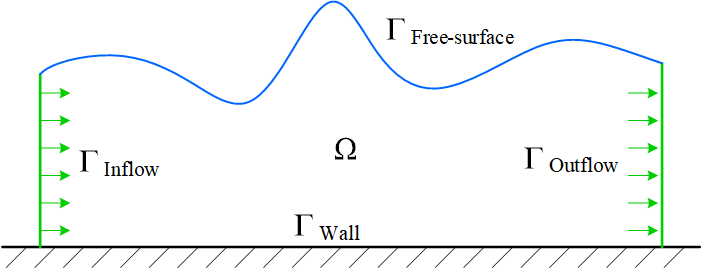
\includegraphics[width=0.6\textwidth]{figures/ch2-SPH-field.png}
  \caption{SPH流场示意图}
  \label{fig:ch2-SPH-field}
\end{myfigure}

(1)	自由液面边界条件

自由液面运动学边界条件要求初始时刻在自由液面处的流体微团在液面不发生破碎的情况下仍保持在自由液面上，%
即自由液面处流体微团的法向速度与自由液面的法向速度相等：
\begin{equation}
  \bm{u} \cdot \bm{n}_{\Gamma_{\rm{Free-surface}}} %
  = \bm{u}_{\Gamma_{\rm{Free-surface}}} \cdot \bm{n}_{\Gamma_{\rm{Free-surface}}}, %
  \quad \bm{r} \in \Gamma_{\rm{Free-surface}}
\end{equation}
式中：$\bm{u}$和$\bm{u}_{\Gamma_{\rm{Free-surface}}}$分别为流体微团和自由液面的速度，%
$\bm{n}_{\Gamma_{\rm{Free-surface}}}$为自由液面的外法向。

自由液面动力学边界条件在不考虑表面张力时，要求在跨越自由表面时的压力连续。%
在本文中不考虑气相的影响，因此可以认为自由液面处的压力为$p = 0$。%
由于在SPH方法中压力通过状态方程求解，因此自由液面处的密度为$\rho = \rho_0$。%
从而动力学边界条件可以写为：
\begin{equation}
  \nabla \cdot \bm{u} = -\frac{1}{\rho} \frac{{\rm{D}}\rho}{{\rm{D}}t} = 0, %
  \quad \bm{r} \in \Gamma_{\rm{Free-surface}}
\end{equation}

由于SPH方法是拉格朗日方法，因此自由液面运动学边界条件能够被隐式满足。%
而对于弱可压SPH方法，如果采用合适的离散格式\cite{colagrossiTheoreticalConsiderationsFreesurface2009}，%
自由液面动力学边界条件也可以被隐式满足。%
因此在$\delta^+$-SPH模型中无需额外处理即可隐式满足自由液面边界条件，这也是该方法适合于模拟自由液面流动的主要原因之一。

(2)	固壁边界条件%

固壁边界处首先需要满足无穿透条件，并且根据是否考虑壁面的粘性力作用可以分为无滑移和自由滑移这两种边界条件。%
由于在本文所涉及的波浪与结构物相互作用问题中，流体对结构物的粘性力作用远小于压力作用，%
因此可以忽略壁面粘性作用而采用自由滑移边界条件：
\begin{equation}
  \bm{u} \cdot \bm{n}_{\Gamma_{\rm{Wall}}} %
  = \bm{u}_{\Gamma_{\rm{Wall}}} \cdot \bm{n}_{\Gamma_{\rm{Wall}}}, %
  \quad \bm{r} \in \Gamma_{\rm{Wall}}
\end{equation}
式中：$\bm{n}_{\Gamma_{\rm{Wall}}}$和$\bm{u}_{\Gamma_{\rm{Wall}}}$分别为壁面的速度和外法向。

本文针对固壁边界条件的处理采用了固定虚粒子边界技术\cite{marroneDSPHModelSimulating2011,adamiGeneralizedWallBoundary2012}，%
该边界技术相较于排斥力边界法\cite{monaghanSimulatingFreeSurface1994}对壁面压力的计算更为精确。%
在固定虚粒子边界技术中，壁面被离散为一组相对位置不发生变化的虚粒子，%
其压力、速度等物理量可以由流体粒子直接插值得出，因此对于不规则边界的适应性较好。%
在SPH计算中，虚粒子被作为固定的流体粒子参与连续性方程和动量方程的求解。%
当流体粒子向壁面运动时其密度增大，所受的压力也相应增大，从而阻止流体粒子穿透壁面，隐式地满足了无穿透条件。%

(3)	流入流出边界条件%

一般而言流入边界处需要提供速度和压力作为边界条件，%
而流出边界处既可施加压力或速度边界条件，也可施加自由流出边界条件。%
由于在本文所构建的势粘流耦合模型中，势流区域和SPH粘流区域间会发生流入流出，%
因此流入流出边界条件会在后文势粘流耦合模型的介绍中详细说明。

\subsubsection{
  \texorpdfstring{数值消波} % 正文和目录中显示的标题
  {\thesubsubsection 数值消波} % 书签页中显示的标题
}
\label{sssec:数值消波}

一般在SPH方法中可以通过简单地增大局部区域的人工粘性，从而加快动能在该区域内的耗散以实现消波。%
但这种通过耗散的消波方法效果有限，因此这里采用了一种在动量方程中引入源项的消波方法\cite{renNonlinearSimulationsWaveinduced2015}，%
能够更加高效地实现消波功能。引入源项后的动量方程如下：
\begin{equation}
  \left\{
    \begin{aligned}
      & \left(\frac{{\rm{D}}\bm{u}_i}{{\rm{D}}t}\right)_{\rm{Absorbing}} = %
      \left(\frac{{\rm{D}}\bm{u}_i}{{\rm{D}}t}\right)_{\rm{SPH}} - \zeta \left(x_i\right)\bm{u}_i \\
      & \zeta\left(x_i\right) = C_0 \frac{\left| x_i - x_0 \right|}{L_{\rm{Absorbing}}}
    \end{aligned}
  \right., %
  \quad \bm{r}_i \in \Omega_{\rm{Absorbing}}
\end{equation}
式中：$\left({\rm{D}}\bm{u}_i/{\rm{D}}t\right)_{\rm{SPH}}$为\cref{eq:DSPH-discrete}中动量方程的左端项，%
$\Omega_{\rm{Absorbing}}$表示消波区域，$x_0$为消波区域的起点坐标。%
$\zeta_0$为影响消波效果的参数，本文计算中参考文献\parencite{renNonlinearSimulationsWaveinduced2015}取为$\zeta_0 = 4.0$。

\subsubsection{
  \texorpdfstring{时间积分} % 正文和目录中显示的标题
  {\thesubsubsection 时间积分} % 书签页中显示的标题
}
\label{sssec:时间积分}

本文中SPH方法所采用的时间积分策略为四阶Runge-Kutta格式(简称RK4)。%
时间步长$\Delta t$受到流体粘度、最大速度、最大加速度和声阻尼系数的约束\cite{antuonoEnergyBalanceDSPH2015,sunInclusionAcousticDamper2023}：
\begin{equation}
  \left\{
    \begin{aligned}
      & \Delta t_{\nu} = 0.125 \frac{h^2}{\nu}, \quad %
      \Delta t_a = 0.25 \min_i\sqrt{\frac{h}{\left|\bm{a}_i\right|}} \\
      & \Delta t_c = {\rm{CFL}}\min_i\frac{h}{c_0 + \left|\bm{u}_i\right|}, \quad %
      \Delta t_{ad} = \frac{{\rm{CFL}}}{\alpha_2}\min_i\frac{h}{c_0 + \left|\bm{u}_i\right|} \\
      & \Delta t = \min\left(\Delta t_{\nu},\Delta t_a,\Delta t_c,\Delta t_{ad}\right)
    \end{aligned}
  \right.
\end{equation}
式中：$\nu$为流体的运动粘性系数。在本文SPH计算中的CFL数均取为1.25以保证计算的收敛性。

\subsection{
  \texorpdfstring{求解器验证及收敛性分析} % 正文和目录中显示的标题
  {\thesubsection 求解器验证及收敛性分析} % 书签页中显示的标题
}
\label{ssec:求解器验证及收敛性分析}

为了验证三类方法的收敛性和准确性，%
本节参考文献中活塞式造波机波浪水槽的造波试验\cite{HuangJiYuXiuZhengGuangHuaLiZiLiuTi2022}，%
采用开源软件HOS-NWT以及自主开发的BEM和SPH求解器进行了数值波浪模拟。%
数值波浪模拟的参数设置在\cref{tab:ch2-wave-setup}中给出，%
不规则波的造波机位移时程曲线在\cref{fig:ch2-wave-setup-irpaddle}中给出。%
对照试验中的设置，在数值水池中布置了波高测点$x_{\rm{probe1}} = 2.37m$和%
$x_{\rm{probe2} = 6.37m}$，如\cref{fig:ch2-wave-setup}所示。%
在每种方法的数值水池末端均采用了消波手段以消除反射波的影响，其中消波区域的长度均为$L_{\rm{Absorbing}} = 0.2L$。%
\begin{mytable}
  \caption{数值波浪模拟参数设置}
  \label{tab:ch2-wave-setup}
  \begin{tabularx}{\textwidth}{*6{>{\centering\arraybackslash}X}}
    \toprule
    {波浪类型} & {周期($T$/s)} & {波幅($A$/m)} & {水深($d$/m)} & {水池长度($L$/m)} & {模拟时长($t_s$/s)} \\
    \midrule
    {规则波} & {1.0} & {0.02} & {0.266} & {30.0} & {30.0} \\
    {不规则波} & {——} & {——} & {0.263} & {30.0} & {60.0} \\
    \bottomrule
  \end{tabularx}
\end{mytable}
\begin{myfigure}
  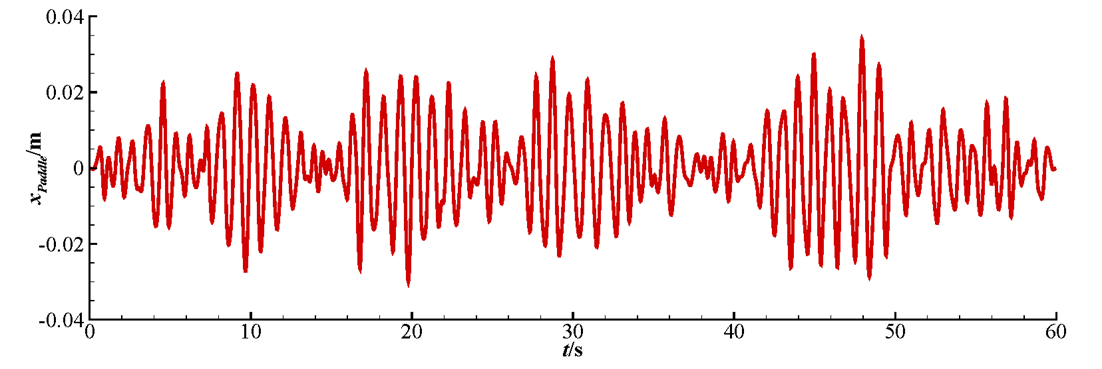
\includegraphics[width=0.8\textwidth]{figures/ch2-wave-setup-irpaddle.png}
  \caption{不规则波的造波机位移时程曲线}
  \label{fig:ch2-wave-setup-irpaddle}
\end{myfigure}
\begin{myfigure}
  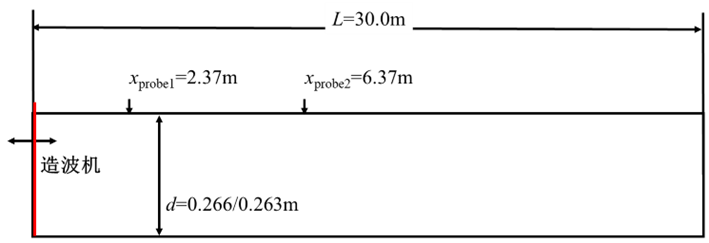
\includegraphics[width=0.8\textwidth]{figures/ch2-wave-setup.png}
  \caption{数值波浪模拟水池设置}
  \label{fig:ch2-wave-setup}
\end{myfigure}

\subsubsection{
  \texorpdfstring{HOS求解器验证} % 正文和目录中显示的标题
  {\thesubsubsection HOS求解器验证} % 书签页中显示的标题
}
\label{sssec:HOS求解器验证}

HOS-NWT在模拟波浪时，对于二维问题需要设置的计算参数主要有以下几个：%
SWEET模型的非线性阶数$i_{\rm{wmk}}$、摄动展开阶数$m_{\rm{HOS}}$、%
波浪场$x$方向上的模态阶数$n_1$和造波机模态阶数$n_3$，%
其中模态数$n_1$和$n_3$一般选取为$(2^k + 1)$，%
更多细节请参考文献\parencite{ducrozetModifiedHighOrderSpectral2012}。%
在本小节的数值波浪模拟中，部分参数参考文献\cite{ducrozetModifiedHighOrderSpectral2012}分别设置为：%
$i_{\rm{wmk}} = 1$，$m_{\rm{HOS}} = 3$，$n_3 = 33$。%
由于$x$方向上模态阶数$n_1$的选取对结果影响较大，下面对其进行收敛性分析，%
分别选取$n_1$为129，257，513和1025进行计算。%
\cref{fig:ch2-wave-HOS-probe1}和\cref{fig:ch2-wave-HOS-probe2}分别给出了在不同参数设置下，%
测点$x_{\rm{probe1}}$和$x_{\rm{probe2}}$处规则波和不规则波的波高结果对比。
\begin{myfigure}
  \begin{subfigure}[b]{0.8\textwidth}
    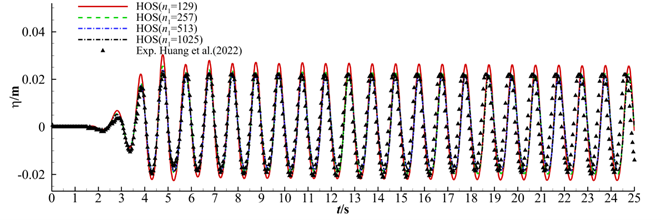
\includegraphics[width=\textwidth]{figures/ch2-wave-HOS-re-probe1.png}
    \caption{规则波}
    \label{ch2-wave-HOS-re-probe1}
  \end{subfigure}
  \begin{subfigure}[b]{0.8\textwidth}
    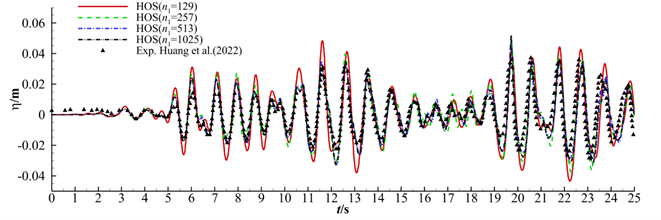
\includegraphics[width=\textwidth]{figures/ch2-wave-HOS-ir-probe1.png}
    \caption{不规则波}
    \label{ch2-wave-HOS-ir-probe1}
  \end{subfigure}
  \caption{$x_{\rm{probe1}}$处的波高：HOS方法结果与文献中试验结果\cite{HuangJiYuXiuZhengGuangHuaLiZiLiuTi2022}对比}
  \label{fig:ch2-wave-HOS-probe1}
\end{myfigure}
\begin{myfigure}
  \begin{subfigure}[b]{0.8\textwidth}
    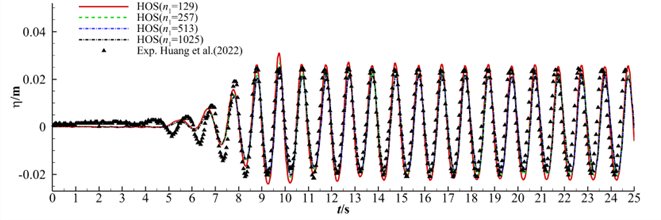
\includegraphics[width=\textwidth]{figures/ch2-wave-HOS-re-probe2.png}
    \caption{规则波}
    \label{ch2-wave-HOS-re-probe2}
  \end{subfigure}
  \begin{subfigure}[b]{0.8\textwidth}
    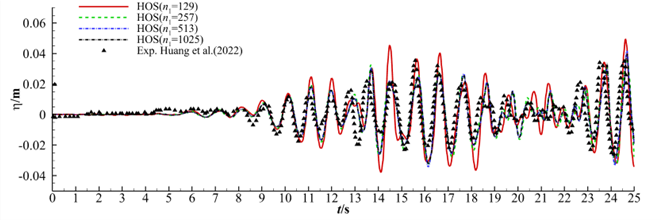
\includegraphics[width=\textwidth]{figures/ch2-wave-HOS-ir-probe2.png}
    \caption{不规则波}
    \label{ch2-wave-HOS-ir-probe2}
  \end{subfigure}
  \caption{$x_{\rm{probe2}}$处的波高：HOS方法结果与文献中试验结果\cite{HuangJiYuXiuZhengGuangHuaLiZiLiuTi2022}对比}
  \label{fig:ch2-wave-HOS-probe2}
\end{myfigure}
\begin{mytable}
  \caption{规则波算例中HOS方法在测点$x_{\rm{probe1}}$处的平均波高对比}
  \label{tab:ch2-wave-HOS-re}
  \begin{tabularx}{\textwidth}{*6{>{\centering\arraybackslash}X}}
    \toprule
    & \multirow{2}{*}{$\bar{\eta}_{\rm{The}}$} & \multicolumn{4}{c}{HOS($n_1$)} \\
    \cline{3-6}
    & & {129} & {257} & {513} & {1025} \\
    \midrule
    {$\bar{\eta}$/m} & {0.04} & {0.04865} & {0.04253} & {0.04053} & {0.04018} \\
    {$\epsilon$/\%} & {——} & {21.63} & {6.33} & {1.33} & {0.45} \\
    \bottomrule
  \end{tabularx}
\end{mytable}

\cref{tab:ch2-wave-HOS-re}中给出了规则波算例中HOS方法结果在测点$x_{\rm{probe1}} = 2.37m$处的平均波高对比，%
其中$\epsilon = \left|\bar{\eta} - \bar{\eta}_{\rm{The}}/\bar{\eta}_{\rm{The}} \times 100\%\right|$，%
$\bar{\eta}$和$\bar{\eta}_{\rm{The}}$分别为HOS方法和理论值在测点处的平均波高。%
结合图表结果可以看出，在规则波算例中随着$n_1$取值增大，%
平均波高逐渐收敛于$\bar{\eta}_{\rm{The}}$，并且当$n_1 = 513$时基本已经收敛。%
从图中不规则波的波高结果中可以看出，当$n_1 = 513$时也基本已经收敛。%

从图表中可以看出HOS方法在模拟规则波和不规则波时，结果收敛后与试验结果吻合比较良好。%
虽然由于其势流方法低数值耗散的特性，在不规则波结果中偶尔会出现波幅略大的情况，但并不影响整体结果的准确性。%
此外需要额外说明，\cref{fig:ch2-wave-HOS-probe1}和\cref{fig:ch2-wave-HOS-probe2}中试验结果随着时间推移逐渐出现了相位偏差，%
这是由于试验过程中的消波处理不够彻底所导致的反射波略微影响了试验结果\cite{HuangJiYuXiuZhengGuangHuaLiZiLiuTi2022}。